% kuleuventheme2 by Janez Kren, September 2017, janez.kren@kuleuven.be, based on:
% kuleuventheme 1.3 by Roland Pastorino, 2013 roland.pastorino@kuleuven.be / www.rolandpastorino.com

\documentclass[11pt,t]{beamer}
\usetheme{kuleuven2}	%THEME OPTIONS for LOGO: kul (default), kulak, lrd,    ; OPTIONS for TITLE PAGE: normal (default), sedes


%%% OTHER SETTINGS
\usefonttheme[onlymath]{serif}			% math font with serifs, delete to make it sans-serif
\setbeamertemplate{footline}[body] 		% delete this line to remove footline bar on all frames
\usepackage[orientation=landscape,size=custom,width=16,height=9,scale=0.5,debug]{beamerposter} %enable for widescreen 16:9 ratio
%\titlegraphic{ \includegraphics[width=.2\paperwidth]{mytitlepagepic.png} } %optional title page image


%%% ADDED PACKAGES:
\usepackage[english]{babel}
\usepackage{amsfonts}
\usepackage{amssymb}


%%% TITLE PAGE INFO:
\title[Distributed Adversarial Attacks]{Evasive and efficient distributed adversarial attacks using PSO} %[]] will appear in footline
\subtitle{Intermediate presentation}

\author{Sander Prenen}
\date{Mentors: I. Tsingenopoulos, V. Rimmer}
\institute{Thesis~supervisors:~Prof.~dr.~ir.~W.~Joosen,~Dr.~ir.~D.~Preuveneers}




\begin{document}
\csname beamer@calculateheadfoot\endcsname %recalculate head and foot dimension

% Title page
\begin{frame}[plain,noframenumbering]
	\titlepage
\end{frame}

% Table of Contents
\begin{frame}{Outline}
	\hfill	{\large \parbox{.961\textwidth}{\tableofcontents[hideothersubsections]}}
\end{frame}

\section{Background \& related work}
\begin{frame}{Adversarial Attacks}
\begin{quote}
Imperceptibly small perturbations to a correctly classified input image, so that it is no longer classified correctly. \cite{szegedy2014intriguing}
\end{quote}

\begin{itemize}
	\item White box attacks
	\item Black box attacks
	\begin{itemize}
		\item Subset of white box attacks
		\item More relevant in security use-cases
		\begin{itemize}
			\item Bypassing malware detection \cite{malware_detection}
			\item Bypassing face recognition \cite{face_recognition}
			\item Altering traffic signs \cite{traffic_signs}
		\end{itemize}		 
	\end{itemize}
\end{itemize}
\end{frame}


%% Boundary Attack
\begin{frame}{Related work}
\begin{itemize}
	\item Boundary attack (BA)
	\vspace{-32pt}
	\hspace{5pt}
	\begin{figure}
	\centering
	\hspace{5pt}
	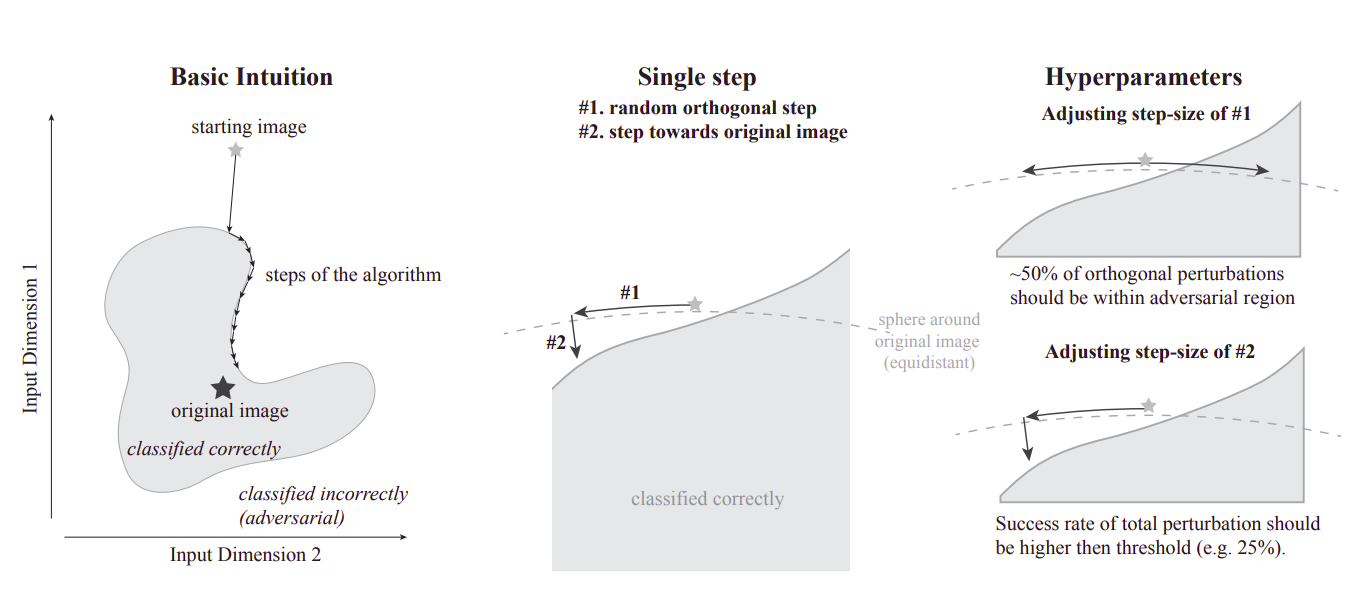
\includegraphics[width=0.4\textwidth]{graphics/boundary_attack.png}
	\caption{Boundary attack \cite{brendel2018decisionbased}\label{fig:boundary_attack}}
	\footnotesize
	\flushleft
	\end{figure}
\end{itemize}

\end{frame}

%%% Biased Boundary Attack
%\begin{frame}{Related work}
%\begin{itemize}
%	\item Boundary attack (BA)
%	\item Biased boundary Attack (BBA)
%	\begin{itemize}
%		\item Masking
%		\item Perlin noise
%	\end{itemize}
%\end{itemize}
%\end{frame}
%
%% HopSkipJump Attack
\begin{frame}{Related work}
\begin{itemize}
	\item HopSkipJump attack (HSJA)
	\vspace{6pt}
	\begin{figure}
	\centering
	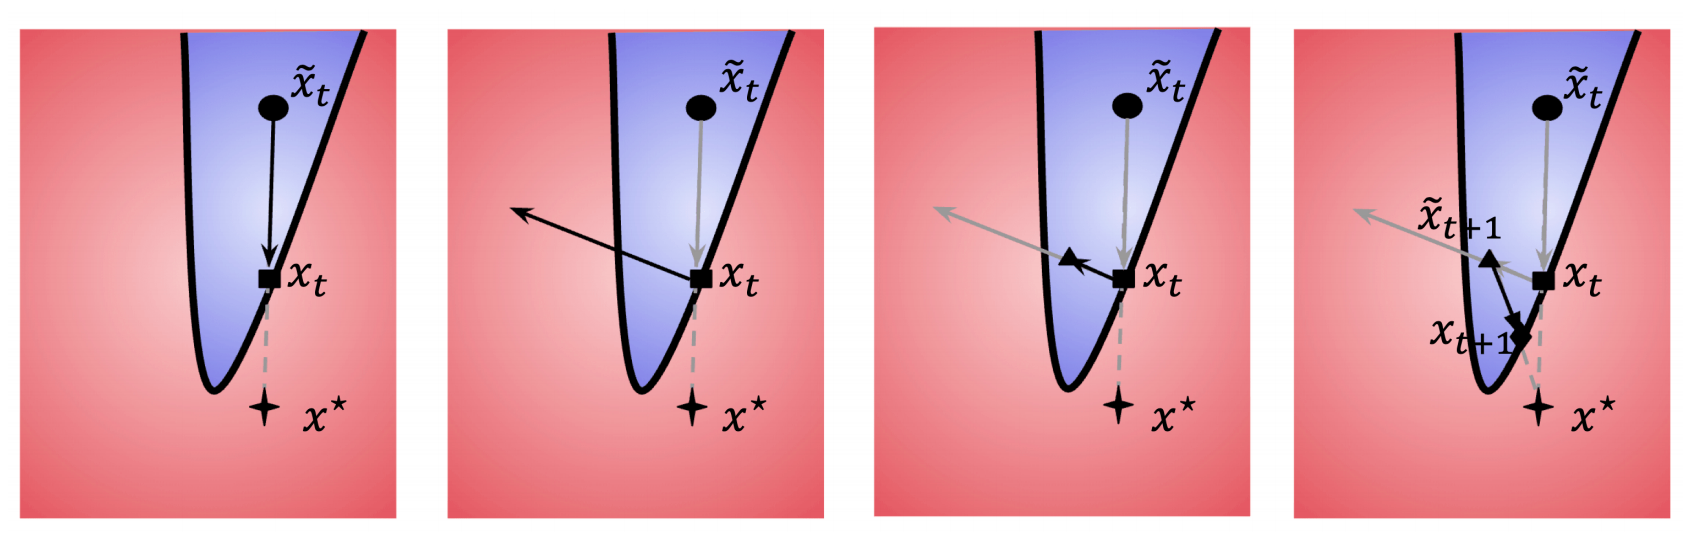
\includegraphics[width=0.8\textwidth]{graphics/hsj_attack.png}
	\caption{HopSkipJump attack \cite{chen2020hopskipjumpattack}\label{fig:hsj_attack}}
	\footnotesize
	\flushleft
	\end{figure}
\end{itemize}
\end{frame}

\begin{frame}{Adversarial Defenses}
\begin{itemize}
	\item Adversarial training
	\item Gradient hiding
	\item Denoising
\end{itemize}

\end{frame}

\begin{frame}{Related work}
	\begin{itemize}
	\item Stateful detection
	
	\onslide<1>
		\begin{figure}
		\centering
		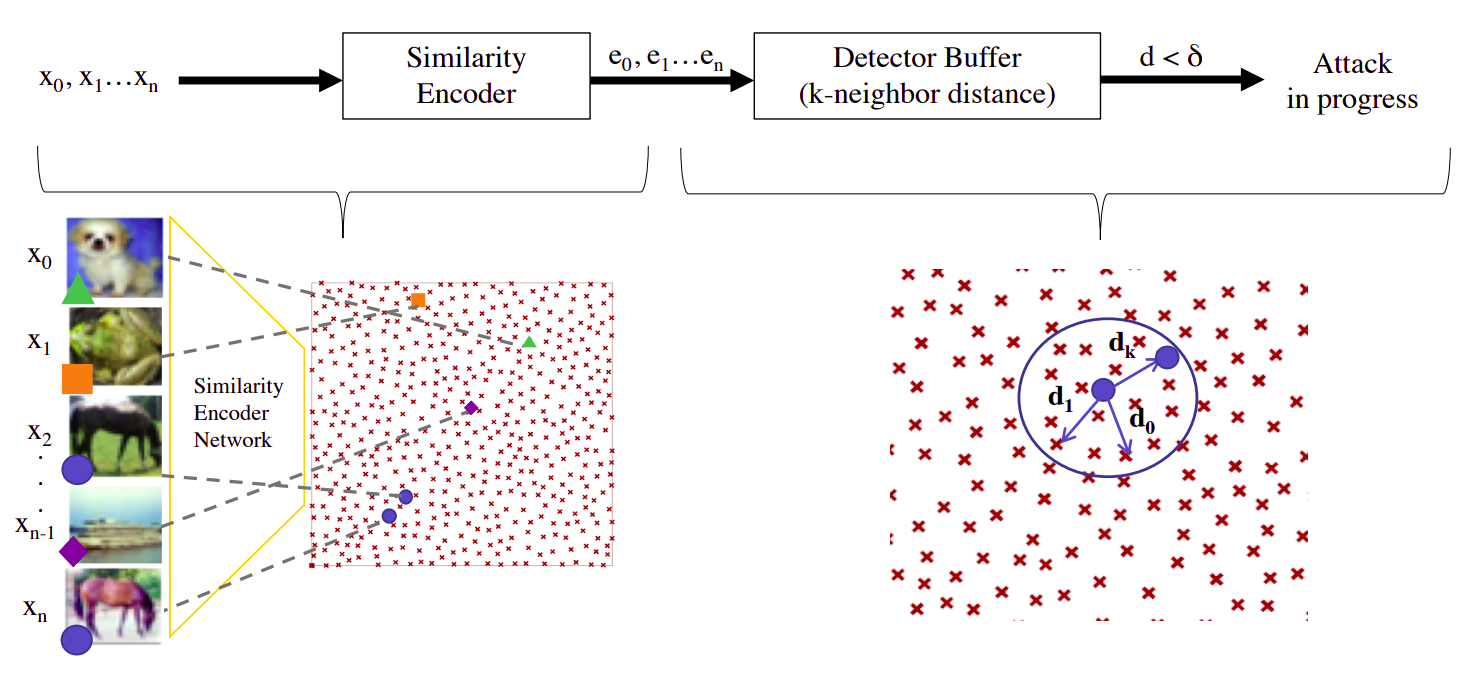
\includegraphics[width=0.8\textwidth]{graphics/stateful_detection.png}
		\caption{Stateful detection \cite{chen2019stateful}	
		\label{fig:stateful_detection}}
		\footnotesize
		\flushleft
		\end{figure}
	\end{itemize}
\end{frame}

\begin{frame}{Related work}
\begin{itemize}
	\item Stateful detection
	\begin{itemize}
		\item Assumption: attack done by \alert{one} user/account/IP
		\item User can be uniquely identified
		\item No cooperation between users
	\end{itemize}
\end{itemize}
\end{frame}

\subsection{Related work}
%% Particle Swarm Optimization
\begin{frame}{Particle Swarm Optimization (PSO)}
\begin{itemize}
	\item Evolutionary algorithm
	\item Optimization framework
	\item Inspired by flocking of birds
	\begin{itemize}
		\item Each particle has a position and corresponding fitness
		\item Move based on personal best position, group best position and inertia 
	\end{itemize}
\end{itemize}
	\tikzset{every picture/.style={line width=0.75pt}} %set default line width to 0.75pt  
	      
\begin{figure}
\centering
\scalebox{0.5}{%
\begin{tikzpicture}[x=0.75pt,y=0.75pt,yscale=-1,xscale=1]

%uncomment if require: \path (0,300); %set diagram left start at 0, and has height of 300

%Shape: Circle [id:dp06935534605548432] 
\draw  [fill={rgb, 255:red, 0; green, 0; blue, 0 }  ,fill opacity=1 ] (100,161) .. controls (100,152.16) and (107.16,145) .. (116,145) .. controls (124.84,145) and (132,152.16) .. (132,161) .. controls (132,169.84) and (124.84,177) .. (116,177) .. controls (107.16,177) and (100,169.84) .. (100,161) -- cycle ;
%Straight Lines [id:da36297070749556615] 
\draw [color={rgb, 255:red, 255; green, 0; blue, 0 }  ,draw opacity=1 ][line width=3]    (116,161) -- (109.44,250.02) ;
\draw [shift={(109,256)}, rotate = 274.21] [fill={rgb, 255:red, 255; green, 0; blue, 0 }  ,fill opacity=1 ][line width=0.08]  [draw opacity=0] (16.97,-8.15) -- (0,0) -- (16.97,8.15) -- cycle    ;
%Shape: Circle [id:dp2975589876543052] 
\draw  [fill={rgb, 255:red, 0; green, 0; blue, 0 }  ,fill opacity=1 ] (258,156) .. controls (258,147.16) and (265.16,140) .. (274,140) .. controls (282.84,140) and (290,147.16) .. (290,156) .. controls (290,164.84) and (282.84,172) .. (274,172) .. controls (265.16,172) and (258,164.84) .. (258,156) -- cycle ;
%Straight Lines [id:da11974704599725938] 
\draw [color={rgb, 255:red, 255; green, 0; blue, 0 }  ,draw opacity=1 ][line width=3]    (274,156) -- (267.44,245.02) ;
\draw [shift={(267,251)}, rotate = 274.21] [fill={rgb, 255:red, 255; green, 0; blue, 0 }  ,fill opacity=1 ][line width=0.08]  [draw opacity=0] (16.97,-8.15) -- (0,0) -- (16.97,8.15) -- cycle    ;
%Straight Lines [id:da34669530870861953] 
\draw [color={rgb, 255:red, 0; green, 0; blue, 255 }  ,draw opacity=1 ][line width=3]    (267,251) -- (207.74,176.69) ;
\draw [shift={(204,172)}, rotate = 51.43] [fill={rgb, 255:red, 0; green, 0; blue, 255 }  ,fill opacity=1 ][line width=0.08]  [draw opacity=0] (16.97,-8.15) -- (0,0) -- (16.97,8.15) -- cycle    ;
%Straight Lines [id:da2944239439562262] 
\draw [color={rgb, 255:red, 55; green, 158; blue, 54 }  ,draw opacity=1 ][line width=3]    (204,172) -- (217.97,148.18) ;
\draw [shift={(221,143)}, rotate = 120.38] [fill={rgb, 255:red, 55; green, 158; blue, 54 }  ,fill opacity=1 ][line width=0.08]  [draw opacity=0] (16.97,-8.15) -- (0,0) -- (16.97,8.15) -- cycle    ;
%Straight Lines [id:da9472051718664152] 
\draw [color={rgb, 255:red, 243; green, 0; blue, 255 }  ,draw opacity=1 ][line width=2.25]  [dash pattern={on 2.53pt off 3.02pt}]  (274,156) -- (224.88,143.95) ;
\draw [shift={(221,143)}, rotate = 13.78] [color={rgb, 255:red, 243; green, 0; blue, 255 }  ,draw opacity=1 ][line width=2.25]    (15.74,-7.06) .. controls (10.01,-3.31) and (4.76,-0.96) .. (0,0) .. controls (4.76,0.96) and (10.01,3.31) .. (15.74,7.06)   ;
%Straight Lines [id:da8503925276289086] 
\draw [color={rgb, 255:red, 0; green, 0; blue, 255 }  ,draw opacity=1 ][line width=3]    (116,161) -- (56.74,86.69) ;
\draw [shift={(53,82)}, rotate = 51.43] [fill={rgb, 255:red, 0; green, 0; blue, 255 }  ,fill opacity=1 ][line width=0.08]  [draw opacity=0] (16.97,-8.15) -- (0,0) -- (16.97,8.15) -- cycle    ;
%Straight Lines [id:da10251717157021911] 
\draw [color={rgb, 255:red, 55; green, 158; blue, 54 }  ,draw opacity=1 ][line width=3]    (116,161) -- (129.97,137.18) ;
\draw [shift={(133,132)}, rotate = 120.38] [fill={rgb, 255:red, 55; green, 158; blue, 54 }  ,fill opacity=1 ][line width=0.08]  [draw opacity=0] (16.97,-8.15) -- (0,0) -- (16.97,8.15) -- cycle    ;

% Text Node
\draw (46,156) node [anchor=north west][inner sep=0.75pt]   [align=left] {Particle};
% Text Node
\draw (115,244) node [anchor=north west][inner sep=0.75pt]   [align=left] {\textcolor[rgb]{1,0,0}{Inertia}};
% Text Node
\draw (38,65) node [anchor=north west][inner sep=0.75pt]  [color={rgb, 255:red, 0; green, 0; blue, 255 }  ,opacity=1 ] [align=left] {Swarm best};
% Text Node
\draw (94,110) node [anchor=north west][inner sep=0.75pt]  [color={rgb, 255:red, 55; green, 158; blue, 54 }  ,opacity=1 ] [align=left] {Individual best};
% Text Node
\draw (212,117) node [anchor=north west][inner sep=0.75pt]   [align=left] {\textcolor[rgb]{0.95,0,1}{New position}};


\end{tikzpicture}
}
\caption{PSO logic, inspired by \cite{pso}}
\label{fig:pso}
\end{figure}
\end{frame}


\section{Research topic}
\begin{frame}{Research topic}
\begin{itemize}
	\item Evasive and Efficient Attacks
	\begin{itemize}
		\item Evade stateful defense
		\item By being efficient (less queries)
		\item By distribution
	\end{itemize}
	\item Distribution
	\begin{itemize}
		\item Centralize the algorithm 
		\item Distribute the submission of queries
		\item Distribute points of attack
	\end{itemize}
\end{itemize}
\end{frame}


%\begin{frame}{Adversarial attack}
%\begin{itemize}
%	\item Untargeted attack
%	\begin{itemize}
%		\item Misclassify to \alert{any} label
%		\item Easier to create adversarial examples
%	\end{itemize}
%	\item Targeted attack
%	\begin{itemize}
%		\item Misclassify to \alert{specific} label
%		\item More relevant in real scenarios
%	\end{itemize}
%\end{itemize}
%\end{frame}

\subsection{Research gap}
\begin{frame}{Research gap}
\begin{itemize}	
	\item Distribution
	\begin{itemize}
		\item Dual goal
		\begin{itemize}
			\item Evade detection
			\item Improve existing attacks using PSO
		\end{itemize}
	\end{itemize}
	
	\item Existing work
	\begin{itemize}
		\item Uses PSO as algorithm in itself
		\item Does not evaluate against stateful detection 
		\item Uses confidence scores \cite{10.1007/978-3-030-59013-0_22, s20247158}
	\end{itemize}
\end{itemize}
\end{frame}

\subsection{Research questions}
\begin{frame}{Possible research questions}
\begin{exampleblock}
	{What are the advantages of distributing an adversarial attack?}
	\end{exampleblock}
	
	\begin{exampleblock}
	{How can attackers cooperate in order to evade a stateful detection mechanism?}
	\end{exampleblock}
	
	\begin{exampleblock}
	{What are the (dis)advantages of using PSO in relation to vanilla adversarial attacks?}
	\end{exampleblock}
\end{frame}


\section{Progress}
\begin{frame}{Threat model}
\begin{itemize}
	\item Decision based attack
	\item Targeted attack
	\begin{itemize}
		\item Both are more relevant in real scenarios
	\end{itemize}
	\item Stateful detection mechanism
	\item Goals: evade detection \& craft best adversarial example	
\end{itemize}
\end{frame}

\begin{frame}{Why PSO?}
\begin{figure}
\centering
\scalebox{0.75}{%


\tikzset{every picture/.style={line width=0.75pt}} %set default line width to 0.75pt        

\begin{tikzpicture}[x=0.75pt,y=0.75pt,yscale=-1,xscale=1]
%uncomment if require: \path (0,822); %set diagram left start at 0, and has height of 822

%Shape: Polygon Curved [id:ds1456428573941393] 
\draw  [fill={rgb, 255:red, 204; green, 200; blue, 200 }  ,fill opacity=1 ] (263,37) .. controls (296,21) and (307,83) .. (292,128) .. controls (277,173) and (230,258) .. (195,233) .. controls (160,208) and (210,159) .. (199,124) .. controls (188,89) and (129,85) .. (143,58) .. controls (157,31) and (167.5,33) .. (183,30) .. controls (198.5,27) and (230,53) .. (263,37) -- cycle ;
%Shape: Star [id:dp3849867744811608] 
\draw  [fill={rgb, 255:red, 0; green, 0; blue, 0 }  ,fill opacity=1 ] (203,75) -- (205.35,79.76) -- (210.61,80.53) -- (206.8,84.24) -- (207.7,89.47) -- (203,87) -- (198.3,89.47) -- (199.2,84.24) -- (195.39,80.53) -- (200.65,79.76) -- cycle ;
%Shape: Circle [id:dp31907763528600963] 
\draw  [fill={rgb, 255:red, 0; green, 0; blue, 0 }  ,fill opacity=1 ] (223,17.5) .. controls (223,15.01) and (225.01,13) .. (227.5,13) .. controls (229.99,13) and (232,15.01) .. (232,17.5) .. controls (232,19.99) and (229.99,22) .. (227.5,22) .. controls (225.01,22) and (223,19.99) .. (223,17.5) -- cycle ;

% Text Node
\draw (217,78) node [anchor=north west][inner sep=0.75pt]  [font=\scriptsize] [align=left] {original image};
% Text Node
\draw (199.02,215.83) node [anchor=north west][inner sep=0.75pt]  [rotate=-302.09] [align=left] {\textit{{\fontfamily{pcr}\selectfont {\footnotesize classified correctly}}}};
% Text Node
\draw (10,99) node [anchor=north west][inner sep=0.75pt]   [align=left] {\textit{{\fontfamily{pcr}\selectfont {\footnotesize classified incorrectly}}}\\{\scriptsize {\fontfamily{pcr}\selectfont \textit{	(adversarial)}}}};


\end{tikzpicture}
\hspace{25mm}
\begin{tikzpicture}[x=0.75pt,y=0.75pt,yscale=-1,xscale=1]
%Shape: Polygon Curved [id:ds6899795161684463] 
\draw  [fill={rgb, 255:red, 204; green, 200; blue, 200 }  ,fill opacity=1 ] (263,37) .. controls (296,21) and (307,83) .. (292,128) .. controls (277,173) and (230,258) .. (195,233) .. controls (160,208) and (210,159) .. (199,124) .. controls (188,89) and (129,85) .. (143,58) .. controls (157,31) and (167.5,33) .. (183,30) .. controls (198.5,27) and (230,53) .. (263,37) -- cycle ;
%Shape: Star [id:dp6357983650621859] 
\draw  [fill={rgb, 255:red, 0; green, 0; blue, 0 }  ,fill opacity=1 ] (203,75) -- (205.35,79.76) -- (210.61,80.53) -- (206.8,84.24) -- (207.7,89.47) -- (203,87) -- (198.3,89.47) -- (199.2,84.24) -- (195.39,80.53) -- (200.65,79.76) -- cycle ;
%Shape: Circle [id:dp7318574978177967] 
\draw  [fill={rgb, 255:red, 0; green, 0; blue, 0 }  ,fill opacity=1 ] (86,148.5) .. controls (86,146.01) and (88.01,144) .. (90.5,144) .. controls (92.99,144) and (95,146.01) .. (95,148.5) .. controls (95,150.99) and (92.99,153) .. (90.5,153) .. controls (88.01,153) and (86,150.99) .. (86,148.5) -- cycle ;
%Shape: Circle [id:dp6030233519979631] 
\draw  [fill={rgb, 255:red, 0; green, 0; blue, 0 }  ,fill opacity=1 ] (106,40.5) .. controls (106,38.01) and (108.01,36) .. (110.5,36) .. controls (112.99,36) and (115,38.01) .. (115,40.5) .. controls (115,42.99) and (112.99,45) .. (110.5,45) .. controls (108.01,45) and (106,42.99) .. (106,40.5) -- cycle ;
%Shape: Circle [id:dp3760625427840725] 
\draw  [fill={rgb, 255:red, 0; green, 0; blue, 0 }  ,fill opacity=1 ] (304,181.5) .. controls (304,179.01) and (306.01,177) .. (308.5,177) .. controls (310.99,177) and (313,179.01) .. (313,181.5) .. controls (313,183.99) and (310.99,186) .. (308.5,186) .. controls (306.01,186) and (304,183.99) .. (304,181.5) -- cycle ;
%Shape: Circle [id:dp7407743072708406] 
\draw  [fill={rgb, 255:red, 0; green, 0; blue, 0 }  ,fill opacity=1 ] (329,67.5) .. controls (329,65.01) and (331.01,63) .. (333.5,63) .. controls (335.99,63) and (338,65.01) .. (338,67.5) .. controls (338,69.99) and (335.99,72) .. (333.5,72) .. controls (331.01,72) and (329,69.99) .. (329,67.5) -- cycle ;
%Shape: Circle [id:dp5720364225968828] 
\draw  [fill={rgb, 255:red, 0; green, 0; blue, 0 }  ,fill opacity=1 ] (156,230.5) .. controls (156,228.01) and (158.01,226) .. (160.5,226) .. controls (162.99,226) and (165,228.01) .. (165,230.5) .. controls (165,232.99) and (162.99,235) .. (160.5,235) .. controls (158.01,235) and (156,232.99) .. (156,230.5) -- cycle ;
%Shape: Circle [id:dp8782112370281272] 
\draw  [fill={rgb, 255:red, 0; green, 0; blue, 0 }  ,fill opacity=1 ] (223,17.5) .. controls (223,15.01) and (225.01,13) .. (227.5,13) .. controls (229.99,13) and (232,15.01) .. (232,17.5) .. controls (232,19.99) and (229.99,22) .. (227.5,22) .. controls (225.01,22) and (223,19.99) .. (223,17.5) -- cycle ;
%Shape: Circle [id:dp4450461879827998] 
\draw  [fill={rgb, 255:red, 0; green, 0; blue, 0 }  ,fill opacity=1 ] (263,226.5) .. controls (263,224.01) and (265.01,222) .. (267.5,222) .. controls (269.99,222) and (272,224.01) .. (272,226.5) .. controls (272,228.99) and (269.99,231) .. (267.5,231) .. controls (265.01,231) and (263,228.99) .. (263,226.5) -- cycle ;
%Shape: Circle [id:dp6155338346417736] 
\draw  [fill={rgb, 255:red, 0; green, 0; blue, 0 }  ,fill opacity=1 ] (414,142.5) .. controls (414,140.01) and (416.01,138) .. (418.5,138) .. controls (420.99,138) and (423,140.01) .. (423,142.5) .. controls (423,144.99) and (420.99,147) .. (418.5,147) .. controls (416.01,147) and (414,144.99) .. (414,142.5) -- cycle ;
%Shape: Circle [id:dp5997279239720605] 
\draw  [fill={rgb, 255:red, 0; green, 0; blue, 0 }  ,fill opacity=1 ] (317,125.5) .. controls (317,123.01) and (319.01,121) .. (321.5,121) .. controls (323.99,121) and (326,123.01) .. (326,125.5) .. controls (326,127.99) and (323.99,130) .. (321.5,130) .. controls (319.01,130) and (317,127.99) .. (317,125.5) -- cycle ;
%Shape: Circle [id:dp05434990394410577] 
\draw  [fill={rgb, 255:red, 0; green, 0; blue, 0 }  ,fill opacity=1 ] (130,23.5) .. controls (130,21.01) and (132.01,19) .. (134.5,19) .. controls (136.99,19) and (139,21.01) .. (139,23.5) .. controls (139,25.99) and (136.99,28) .. (134.5,28) .. controls (132.01,28) and (130,25.99) .. (130,23.5) -- cycle ;
%Shape: Circle [id:dp41958200886409136] 
\draw  [fill={rgb, 255:red, 0; green, 0; blue, 0 }  ,fill opacity=1 ] (288,17.5) .. controls (288,15.01) and (290.01,13) .. (292.5,13) .. controls (294.99,13) and (297,15.01) .. (297,17.5) .. controls (297,19.99) and (294.99,22) .. (292.5,22) .. controls (290.01,22) and (288,19.99) .. (288,17.5) -- cycle ;
%Shape: Circle [id:dp7430516298496386] 
\draw  [fill={rgb, 255:red, 0; green, 0; blue, 0 }  ,fill opacity=1 ] (81,234.5) .. controls (81,232.01) and (83.01,230) .. (85.5,230) .. controls (87.99,230) and (90,232.01) .. (90,234.5) .. controls (90,236.99) and (87.99,239) .. (85.5,239) .. controls (83.01,239) and (81,236.99) .. (81,234.5) -- cycle ;
%Shape: Circle [id:dp7241063621158479] 
\draw  [fill={rgb, 255:red, 0; green, 0; blue, 0 }  ,fill opacity=1 ] (324,201.5) .. controls (324,199.01) and (326.01,197) .. (328.5,197) .. controls (330.99,197) and (333,199.01) .. (333,201.5) .. controls (333,203.99) and (330.99,206) .. (328.5,206) .. controls (326.01,206) and (324,203.99) .. (324,201.5) -- cycle ;


% Text Node
\draw (10,99) node [anchor=north west][inner sep=0.75pt]   [align=left] {\textit{{\fontfamily{pcr}\selectfont {\footnotesize classified incorrectly}}}\\{\scriptsize {\fontfamily{pcr}\selectfont \textit{	(adversarial)}}}};
% Text Node
\draw (199.02,215.83) node [anchor=north west][inner sep=0.75pt]  [rotate=-302.09] [align=left] {\textit{{\fontfamily{pcr}\selectfont {\footnotesize classified correctly}}}};
% Text Node
\draw (217,78) node [anchor=north west][inner sep=0.75pt]  [font=\scriptsize] [align=left] {original image};


\end{tikzpicture}
}
\caption{Advantage of PSO, inspired by \cite{brendel2018decisionbased}}
\label{fig:pso_advantage}
\end{figure}
\end{frame}

\begin{frame}{Progress}
\begin{itemize}
	\item Working PSO algorithm based on boundary attack (PSO-BA)
	\begin{figure}
	\centering
	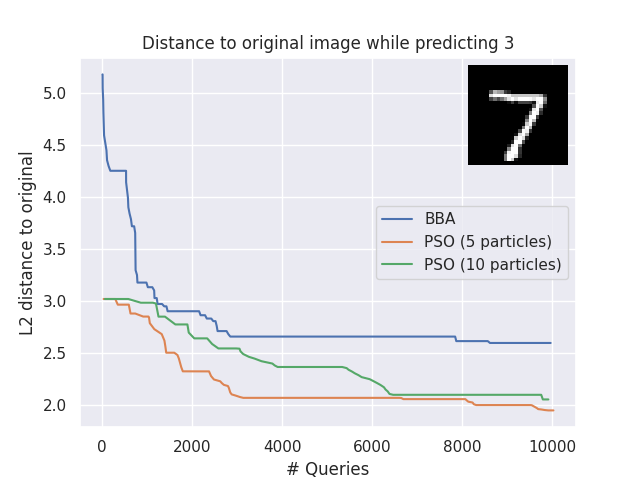
\includegraphics[width=0.45\textwidth]{graphics/comparison_1_3.png}
	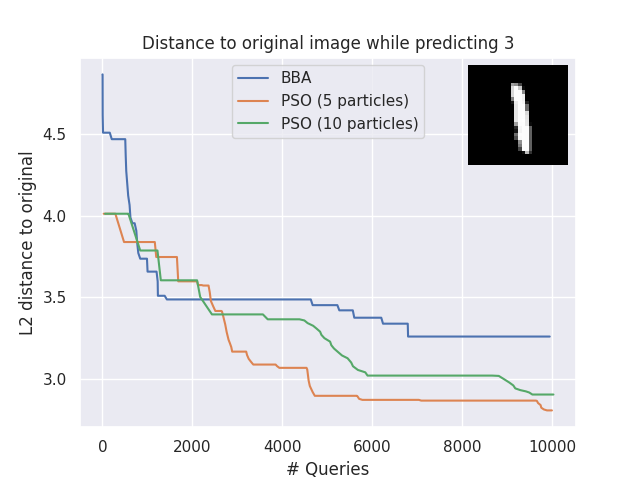
\includegraphics[width=0.45\textwidth]{graphics/comparison_1302_3.png}
	\caption{Comparison BA and PSO-BA\label{fig:comparisons}}
	\footnotesize
	\flushleft
	\end{figure}
\end{itemize}
\end{frame}

\begin{frame}{Why PSO?}
\vspace{-12pt}
\begin{figure}
\centering
\scalebox{0.65}{%
\tikzset{every picture/.style={line width=0.75pt}} %set default line width to 0.75pt             
\begin{tikzpicture}[x=0.75pt,y=0.75pt,yscale=-1,xscale=1]
%uncomment if require: \path (0,243); %set diagram left start at 0, and has height of 243

%Shape: Polygon Curved [id:ds8177605217772814] 
\draw  [fill={rgb, 255:red, 204; green, 200; blue, 200 }  ,fill opacity=1 ] (256,28) .. controls (289,12) and (300,74) .. (285,119) .. controls (270,164) and (223,249) .. (188,224) .. controls (153,199) and (203,150) .. (192,115) .. controls (181,80) and (122,76) .. (136,49) .. controls (150,22) and (160.5,24) .. (176,21) .. controls (191.5,18) and (223,44) .. (256,28) -- cycle ;
%Shape: Star [id:dp4544513566087254] 
\draw  [fill={rgb, 255:red, 0; green, 0; blue, 0 }  ,fill opacity=1 ] (196,66) -- (198.35,70.76) -- (203.61,71.53) -- (199.8,75.24) -- (200.7,80.47) -- (196,78) -- (191.3,80.47) -- (192.2,75.24) -- (188.39,71.53) -- (193.65,70.76) -- cycle ;
%Shape: Circle [id:dp25431166779332526] 
\draw  [fill={rgb, 255:red, 0; green, 0; blue, 0 }  ,fill opacity=1 ] (79,139.5) .. controls (79,137.01) and (81.01,135) .. (83.5,135) .. controls (85.99,135) and (88,137.01) .. (88,139.5) .. controls (88,141.99) and (85.99,144) .. (83.5,144) .. controls (81.01,144) and (79,141.99) .. (79,139.5) -- cycle ;
%Shape: Circle [id:dp04162684077966761] 
\draw  [fill={rgb, 255:red, 255; green, 0; blue, 0 }  ,fill opacity=1 ] (97,30.5) .. controls (97,28.01) and (99.01,26) .. (101.5,26) .. controls (103.99,26) and (106,28.01) .. (106,30.5) .. controls (106,32.99) and (103.99,35) .. (101.5,35) .. controls (99.01,35) and (97,32.99) .. (97,30.5) -- cycle ;
%Shape: Circle [id:dp2703651257399744] 
\draw  [fill={rgb, 255:red, 0; green, 0; blue, 0 }  ,fill opacity=1 ] (297,172.5) .. controls (297,170.01) and (299.01,168) .. (301.5,168) .. controls (303.99,168) and (306,170.01) .. (306,172.5) .. controls (306,174.99) and (303.99,177) .. (301.5,177) .. controls (299.01,177) and (297,174.99) .. (297,172.5) -- cycle ;
%Shape: Circle [id:dp5941926052392863] 
\draw  [fill={rgb, 255:red, 0; green, 0; blue, 0 }  ,fill opacity=1 ] (322,58.5) .. controls (322,56.01) and (324.01,54) .. (326.5,54) .. controls (328.99,54) and (331,56.01) .. (331,58.5) .. controls (331,60.99) and (328.99,63) .. (326.5,63) .. controls (324.01,63) and (322,60.99) .. (322,58.5) -- cycle ;
%Shape: Circle [id:dp2962758051934469] 
\draw  [fill={rgb, 255:red, 0; green, 0; blue, 0 }  ,fill opacity=1 ] (149,221.5) .. controls (149,219.01) and (151.01,217) .. (153.5,217) .. controls (155.99,217) and (158,219.01) .. (158,221.5) .. controls (158,223.99) and (155.99,226) .. (153.5,226) .. controls (151.01,226) and (149,223.99) .. (149,221.5) -- cycle ;
%Shape: Circle [id:dp594888960737932] 
\draw  [fill={rgb, 255:red, 250; green, 0; blue, 0 }  ,fill opacity=1 ] (216,8.5) .. controls (216,6.01) and (218.01,4) .. (220.5,4) .. controls (222.99,4) and (225,6.01) .. (225,8.5) .. controls (225,10.99) and (222.99,13) .. (220.5,13) .. controls (218.01,13) and (216,10.99) .. (216,8.5) -- cycle ;
%Shape: Circle [id:dp9328490781431651] 
\draw  [fill={rgb, 255:red, 0; green, 0; blue, 0 }  ,fill opacity=1 ] (256,217.5) .. controls (256,215.01) and (258.01,213) .. (260.5,213) .. controls (262.99,213) and (265,215.01) .. (265,217.5) .. controls (265,219.99) and (262.99,222) .. (260.5,222) .. controls (258.01,222) and (256,219.99) .. (256,217.5) -- cycle ;
%Shape: Circle [id:dp8990381437523687] 
\draw  [fill={rgb, 255:red, 0; green, 0; blue, 0 }  ,fill opacity=1 ] (407,133.5) .. controls (407,131.01) and (409.01,129) .. (411.5,129) .. controls (413.99,129) and (416,131.01) .. (416,133.5) .. controls (416,135.99) and (413.99,138) .. (411.5,138) .. controls (409.01,138) and (407,135.99) .. (407,133.5) -- cycle ;
%Shape: Circle [id:dp8312522005955618] 
\draw  [fill={rgb, 255:red, 255; green, 0; blue, 0 }  ,fill opacity=1 ] (310,116.5) .. controls (310,114.01) and (312.01,112) .. (314.5,112) .. controls (316.99,112) and (319,114.01) .. (319,116.5) .. controls (319,118.99) and (316.99,121) .. (314.5,121) .. controls (312.01,121) and (310,118.99) .. (310,116.5) -- cycle ;
%Shape: Circle [id:dp9569468228469469] 
\draw  [fill={rgb, 255:red, 255; green, 0; blue, 0 }  ,fill opacity=1 ] (123,14.5) .. controls (123,12.01) and (125.01,10) .. (127.5,10) .. controls (129.99,10) and (132,12.01) .. (132,14.5) .. controls (132,16.99) and (129.99,19) .. (127.5,19) .. controls (125.01,19) and (123,16.99) .. (123,14.5) -- cycle ;
%Shape: Circle [id:dp4374049081512974] 
\draw  [fill={rgb, 255:red, 255; green, 0; blue, 0 }  ,fill opacity=1 ] (281,8.5) .. controls (281,6.01) and (283.01,4) .. (285.5,4) .. controls (287.99,4) and (290,6.01) .. (290,8.5) .. controls (290,10.99) and (287.99,13) .. (285.5,13) .. controls (283.01,13) and (281,10.99) .. (281,8.5) -- cycle ;
%Shape: Circle [id:dp8028138086788923] 
\draw  [fill={rgb, 255:red, 0; green, 0; blue, 0 }  ,fill opacity=1 ] (74,225.5) .. controls (74,223.01) and (76.01,221) .. (78.5,221) .. controls (80.99,221) and (83,223.01) .. (83,225.5) .. controls (83,227.99) and (80.99,230) .. (78.5,230) .. controls (76.01,230) and (74,227.99) .. (74,225.5) -- cycle ;
%Shape: Circle [id:dp8426714491905742] 
\draw  [fill={rgb, 255:red, 0; green, 0; blue, 0 }  ,fill opacity=1 ] (317,192.5) .. controls (317,190.01) and (319.01,188) .. (321.5,188) .. controls (323.99,188) and (326,190.01) .. (326,192.5) .. controls (326,194.99) and (323.99,197) .. (321.5,197) .. controls (319.01,197) and (317,194.99) .. (317,192.5) -- cycle ;
%Shape: Circle [id:dp5447558778664685] 
\draw  [color={rgb, 255:red, 172; green, 172; blue, 172 }  ,draw opacity=1 ][dash pattern={on 4.5pt off 4.5pt}][line width=0.75]  (69.96,74) .. controls (69.96,4.39) and (126.39,-52.04) .. (196,-52.04) .. controls (265.61,-52.04) and (322.04,4.39) .. (322.04,74) .. controls (322.04,143.61) and (265.61,200.04) .. (196,200.04) .. controls (126.39,200.04) and (69.96,143.61) .. (69.96,74) -- cycle ;

% Text Node
\draw (210,69) node [anchor=north west][inner sep=0.75pt]  [font=\scriptsize] [align=left] {original image};
% Text Node
\draw (192.02,206.83) node [anchor=north west][inner sep=0.75pt]  [rotate=-302.09] [align=left] {\textit{{\fontfamily{pcr}\selectfont {\footnotesize classified correctly}}}};
% Text Node
\draw (3,90) node [anchor=north west][inner sep=0.75pt]   [align=left] {\textit{{\fontfamily{pcr}\selectfont {\footnotesize classified incorrectly}}}\\{\scriptsize {\fontfamily{pcr}\selectfont \textit{	(adversarial)}}}};


\end{tikzpicture}
\hspace{8mm}    
\begin{tikzpicture}[x=0.75pt,y=0.75pt,yscale=-1,xscale=1]
%uncomment if require: \path (0,243); %set diagram left start at 0, and has height of 243

%Shape: Polygon Curved [id:ds028311413343864666] 
\draw  [fill={rgb, 255:red, 204; green, 200; blue, 200 }  ,fill opacity=1 ] (256,28) .. controls (289,12) and (300,74) .. (285,119) .. controls (270,164) and (223,249) .. (188,224) .. controls (153,199) and (203,150) .. (192,115) .. controls (181,80) and (122,76) .. (136,49) .. controls (150,22) and (160.5,24) .. (176,21) .. controls (191.5,18) and (223,44) .. (256,28) -- cycle ;
%Shape: Star [id:dp12313301391465115] 
\draw  [fill={rgb, 255:red, 0; green, 0; blue, 0 }  ,fill opacity=1 ] (196,66) -- (198.35,70.76) -- (203.61,71.53) -- (199.8,75.24) -- (200.7,80.47) -- (196,78) -- (191.3,80.47) -- (192.2,75.24) -- (188.39,71.53) -- (193.65,70.76) -- cycle ;
%Shape: Circle [id:dp6155363941380243] 
\draw  [fill={rgb, 255:red, 0; green, 0; blue, 0 }  ,fill opacity=1 ] (79,139.5) .. controls (79,137.01) and (81.01,135) .. (83.5,135) .. controls (85.99,135) and (88,137.01) .. (88,139.5) .. controls (88,141.99) and (85.99,144) .. (83.5,144) .. controls (81.01,144) and (79,141.99) .. (79,139.5) -- cycle ;
%Shape: Circle [id:dp7237584867363258] 
\draw  [fill={rgb, 255:red, 255; green, 0; blue, 0 }  ,fill opacity=1 ] (97,30.5) .. controls (97,28.01) and (99.01,26) .. (101.5,26) .. controls (103.99,26) and (106,28.01) .. (106,30.5) .. controls (106,32.99) and (103.99,35) .. (101.5,35) .. controls (99.01,35) and (97,32.99) .. (97,30.5) -- cycle ;
%Shape: Circle [id:dp3000711687101607] 
\draw  [fill={rgb, 255:red, 255; green, 0; blue, 0 }  ,fill opacity=1 ] (297,172.5) .. controls (297,170.01) and (299.01,168) .. (301.5,168) .. controls (303.99,168) and (306,170.01) .. (306,172.5) .. controls (306,174.99) and (303.99,177) .. (301.5,177) .. controls (299.01,177) and (297,174.99) .. (297,172.5) -- cycle ;
%Shape: Circle [id:dp8075638092808506] 
\draw  [fill={rgb, 255:red, 0; green, 0; blue, 0 }  ,fill opacity=1 ] (322,58.5) .. controls (322,56.01) and (324.01,54) .. (326.5,54) .. controls (328.99,54) and (331,56.01) .. (331,58.5) .. controls (331,60.99) and (328.99,63) .. (326.5,63) .. controls (324.01,63) and (322,60.99) .. (322,58.5) -- cycle ;
%Shape: Circle [id:dp7568424063171841] 
\draw  [fill={rgb, 255:red, 255; green, 0; blue, 0 }  ,fill opacity=1 ] (149,221.5) .. controls (149,219.01) and (151.01,217) .. (153.5,217) .. controls (155.99,217) and (158,219.01) .. (158,221.5) .. controls (158,223.99) and (155.99,226) .. (153.5,226) .. controls (151.01,226) and (149,223.99) .. (149,221.5) -- cycle ;
%Shape: Circle [id:dp061310887713215356] 
\draw  [fill={rgb, 255:red, 250; green, 0; blue, 0 }  ,fill opacity=1 ] (216,8.5) .. controls (216,6.01) and (218.01,4) .. (220.5,4) .. controls (222.99,4) and (225,6.01) .. (225,8.5) .. controls (225,10.99) and (222.99,13) .. (220.5,13) .. controls (218.01,13) and (216,10.99) .. (216,8.5) -- cycle ;
%Shape: Circle [id:dp6007055452606598] 
\draw  [fill={rgb, 255:red, 0; green, 0; blue, 0 }  ,fill opacity=1 ] (256,217.5) .. controls (256,215.01) and (258.01,213) .. (260.5,213) .. controls (262.99,213) and (265,215.01) .. (265,217.5) .. controls (265,219.99) and (262.99,222) .. (260.5,222) .. controls (258.01,222) and (256,219.99) .. (256,217.5) -- cycle ;
%Shape: Circle [id:dp35659310837968516] 
\draw  [fill={rgb, 255:red, 255; green, 0; blue, 0 }  ,fill opacity=1 ] (407,133.5) .. controls (407,131.01) and (409.01,129) .. (411.5,129) .. controls (413.99,129) and (416,131.01) .. (416,133.5) .. controls (416,135.99) and (413.99,138) .. (411.5,138) .. controls (409.01,138) and (407,135.99) .. (407,133.5) -- cycle ;
%Shape: Circle [id:dp051839567624966554] 
\draw  [fill={rgb, 255:red, 0; green, 0; blue, 0 }  ,fill opacity=1 ] (310,116.5) .. controls (310,114.01) and (312.01,112) .. (314.5,112) .. controls (316.99,112) and (319,114.01) .. (319,116.5) .. controls (319,118.99) and (316.99,121) .. (314.5,121) .. controls (312.01,121) and (310,118.99) .. (310,116.5) -- cycle ;
%Shape: Circle [id:dp6100783097259108] 
\draw  [fill={rgb, 255:red, 0; green, 0; blue, 0 }  ,fill opacity=1 ] (123,14.5) .. controls (123,12.01) and (125.01,10) .. (127.5,10) .. controls (129.99,10) and (132,12.01) .. (132,14.5) .. controls (132,16.99) and (129.99,19) .. (127.5,19) .. controls (125.01,19) and (123,16.99) .. (123,14.5) -- cycle ;
%Shape: Circle [id:dp21970625656410747] 
\draw  [fill={rgb, 255:red, 0; green, 0; blue, 0 }  ,fill opacity=1 ] (281,8.5) .. controls (281,6.01) and (283.01,4) .. (285.5,4) .. controls (287.99,4) and (290,6.01) .. (290,8.5) .. controls (290,10.99) and (287.99,13) .. (285.5,13) .. controls (283.01,13) and (281,10.99) .. (281,8.5) -- cycle ;
%Shape: Circle [id:dp7969348915267038] 
\draw  [fill={rgb, 255:red, 0; green, 0; blue, 0 }  ,fill opacity=1 ] (74,225.5) .. controls (74,223.01) and (76.01,221) .. (78.5,221) .. controls (80.99,221) and (83,223.01) .. (83,225.5) .. controls (83,227.99) and (80.99,230) .. (78.5,230) .. controls (76.01,230) and (74,227.99) .. (74,225.5) -- cycle ;
%Shape: Circle [id:dp8807491163133498] 
\draw  [fill={rgb, 255:red, 0; green, 0; blue, 0 }  ,fill opacity=1 ] (317,192.5) .. controls (317,190.01) and (319.01,188) .. (321.5,188) .. controls (323.99,188) and (326,190.01) .. (326,192.5) .. controls (326,194.99) and (323.99,197) .. (321.5,197) .. controls (319.01,197) and (317,194.99) .. (317,192.5) -- cycle ;


% Text Node
\draw (210,69) node [anchor=north west][inner sep=0.75pt]  [font=\scriptsize] [align=left] {original image};
% Text Node
\draw (192.02,206.83) node [anchor=north west][inner sep=0.75pt]  [rotate=-302.09] [align=left] {\textit{{\fontfamily{pcr}\selectfont {\footnotesize classified correctly}}}};
% Text Node
\draw (3,90) node [anchor=north west][inner sep=0.75pt]   [align=left] {\textit{{\fontfamily{pcr}\selectfont {\footnotesize classified incorrectly}}}\\{\scriptsize {\fontfamily{pcr}\selectfont \textit{	(adversarial)}}}};


\end{tikzpicture}
}
\caption{Advantage of PSO, inspired by \cite{brendel2018decisionbased}}
\label{fig:pso_advantage_rand}
\end{figure}
\end{frame}

\begin{frame}[plain]{Progress}
\begin{itemize}
	\item Working PSO algorithm based on boundary attack (PSO-BA)
	\item Performed experiments to show that PSO is a viable candidate
	\begin{figure}
	\centering
	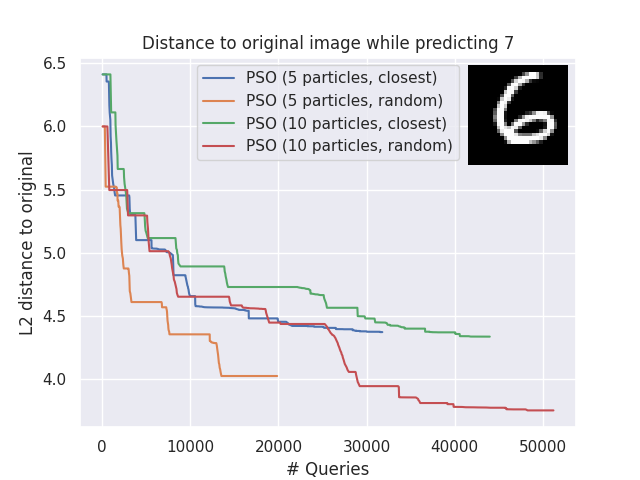
\includegraphics[width=0.45\textwidth]{graphics/random_vs_closest.png}
	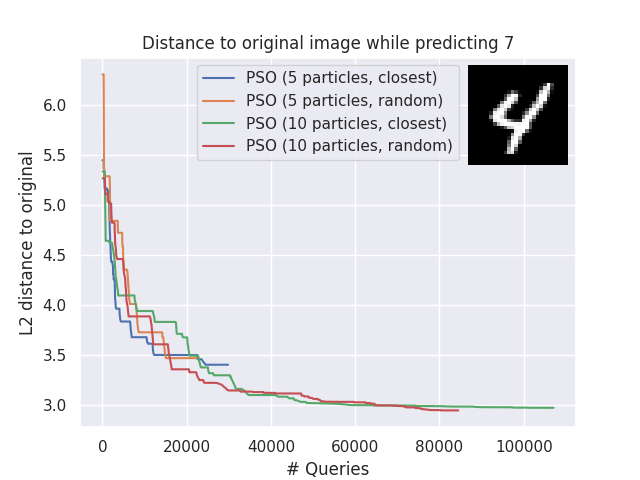
\includegraphics[width=0.45\textwidth]{graphics/random_vs_closest_1.png}
	\caption{Comparison random versus closest initialization\label{fig:rand_vs_close}}
	\footnotesize
	\flushleft
	\end{figure}
\end{itemize}
\end{frame}

\begin{frame}{Progress}
\begin{itemize}
	\item Working PSO algorithm based on boundary attack (PSO-BA)
	\item Performed experiments to show that PSO is a viable candidate
	\item Compare detections PSO-BA and BA
	\begin{table}
		\begin{tabular}{r|c|c|c}
			& Avg. $L_2$-distance & Avg. \# Detections & Avg. \# Queries \\ \hline
		BBA	& 2.9868 &148 &25010 \\
		PSO-BBA & 2.8841	&79	&24721 \\
		D-PSO-BBA & 2.8841 &51 &24721 \\
		\end{tabular}
	\end{table}
\end{itemize}
\end{frame}

\section{Evaluation plan}
\begin{frame}{Next steps}
\begin{itemize}
	\item Improve the existing PSO-BA algorithm
	\item Use different methods of distribution
	\begin{itemize}
		\item Round robin 
		\item Distance based
		\item Other
	\end{itemize}
	\item Implement a new algorithm based on HSJA and PSO
\end{itemize}
\end{frame}

\begin{frame}{Evaluation plan}
\begin{itemize}
	\item Metric: number of detections and $L_2$-distance
	\item Different distribution schemes
	\item Tuning the hyperparameters
	\item Applying the algorithm on different datasets
	\begin{itemize}
		\item CIFAR
		\item ImageNet
	\end{itemize}
	\item Performing more experiments to confirm the results
\end{itemize}
\end{frame}

\begin{frame}[c,plain,noframenumbering]
\begin{tikzpicture}[remember picture,overlay]
\fill[fill=kul-blue]
    (current page.south east)  rectangle  ([shift={(0,-0.1\paperheight)}]current page.north west)   ;
\end{tikzpicture}

\centering
\textcolor{white}{Questions?}
\end{frame}

\appendix
\section*{References}
\begin{frame}[allowframebreaks]{References}
\bibliographystyle{unsrt}
\bibliography{citations.bib}
\end{frame}
\end{document}
